%! Author = giaco
%! Date = 16/05/2024

\chapter{Method}
\label{sec:method}

TODO - WRITE INTRO
% The focus of this work is to simplify as much as possible the representation learning of current RL algorithms leveraging prior knowledge and letting the agent focus on learning the actual policy to solve the task. Our idea is to use \textit{Knowledge Skills}, defined in \ref{sec:skills}, to create a starting point for agents giving them a set of prior knowledge from which they can extract information. Later, as explained in Sec. \ref{sec:extractors}, we tested different ways of concatenating Knowledge Skills before feeding the agents with extracted information.
% The main architecture is depicted in Fig. \ref{fig:main_architecture}.
% The method to train the agent then is divided into two steps.
% First, we created a dataset of game frames as specified in \ref{sec:experiments}, used to pre-train knowledge skills models to learn different structured representations of the input. Then, during RL agent training, we fix the weights of these models and we give the same frame as input to all the skills to extract information and combine them into one single embedding. We then gave this new state representation to the RL agent to learn a policy.

% \begin{figure}[ht]
%     \begin{center}
%         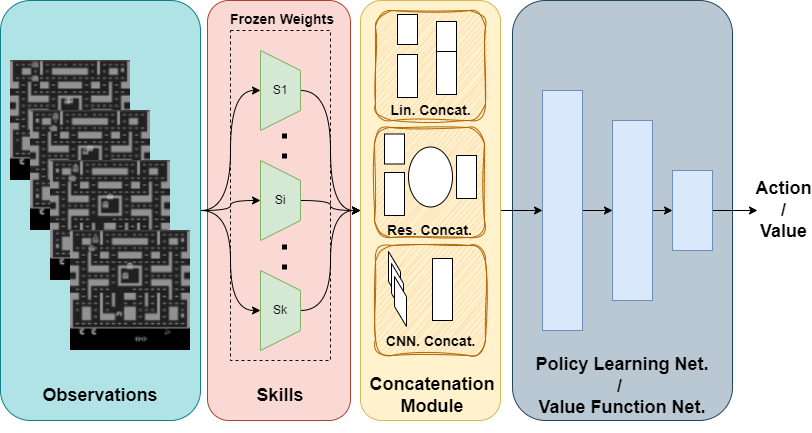
\includegraphics[width=\textwidth]{images/main_architecture.png}
%     \end{center}
%     \caption{In Figure we show a schematic of our proposed architecture. The last four game frames are stacked together and passed as input to all skills.  Given \textit{k} different skills we will have \textit{k} different embeddings. Each of them will be passed as input to a specific extractor. In the figure are shown for simplicity only some of the possible extractors. The extractors will concatenate the information from the different embeddings into a single embedding that will be passed to the network in charge of deciding the action.}
%     \label{fig:main_architecture}
% \end{figure}

\section{Weight Sharing Attention}
\label{sec:wsa}
% Skills can be defined in multiple ways like policies i.e. sequences of actions required to solve a particular task or INSERIRE ALTRI METODI DALLA PROPOSTA DI TESI
% More generally, we refer to \textbf{Knowledge Skills} as components that can encode information. They map the state representation into an enriched latent encoding.
% Formally a \textit{Knowledge Skill K} is defined as a tuple of three different functions $K=<\phi, \gamma, \omega>$:
% \begin{itemize}
%     \item $\phi: \mathbb{R}^{n} \rightarrow \mathbb{R}^{m}$, is the \textit{encoding function}, takes as input a representation and encodes it to apply the skill.

%     \item $\gamma: \mathbb{R}^{n} \rightarrow \mathbb{R}^{m}$, is the \textit{skill function}, applies the skill to the given input.

%     \item $\omega: \mathbb{R}^{n} \rightarrow \mathbb{R}^{m}$, is the \textit{adapter function}, elaborate the output from the skills to make it useful.
% \end{itemize}
% The Knowledge Skills is applied by composing the three functions $K(x) = \omega (\gamma ( \phi(x)))$.
% Specifically, we focused on self-supervised or unsupervised models that solve computer vision tasks. Some of the skills used in this work have already been presented in Sec. \ref{sec:related_work}. We implemented the model in \cite{goel2018unsupervised}, which we called Video Object Segmentation (VOS), to detect moving objects, the model in \cite{kulkarni2019unsupervised}, which we refer as Object Keypoints (OK), to detect keypoints of moving objects on a frame, and finally, we implemented the model of \cite{anand2019unsupervised}, which we called State Representation (SR) to learn the state representation. %rifrasare


% Although very significant, the skills defined up to this point may not provide enough information for the agent to learn. Therefore, we decided to enrich our skill set by using the well-known model based on convolutional layers specified in \cite{mnih2013playing}, which we refer to as \textit{Nature CNN}, as a base architecture to develop other simple skills.
% In fact, Nature CNN has been used in various forms of encoder-decoder to implement: 1) an Autoencoder that takes the last frame of a game, encodes it in a latent space, and then tries to reconstruct the original frame; 2) an Image Completion model that given a frame of a game that is occluded with a black square, tries to reconstruct the original frame without occlusion; 3) finally a Frame Prediction model that given the last four frames of a game, tries to predict and reconstruct the frame 5 steps ahead.
% These last three models were all trained with grayscale game frames of size 84x84 pixels. For the Frame Prediction model, on the other hand, we thought that predicting the frame at the next step might not be very informative since the frame would be very similar to the current one, so we decided to try to predict the frame 5 steps ahead.

%inserire qualche frase in più su come abbiamo create queste ultime 3 skill?, sul perchè abbiamo scelto questi modelli, sul fatto che non soon perfetti in quanto molte volte non predicono bene l'output ma che comunque possono codificare informazioni important per l'agente

% The architecture of Nature CNN has been slightly modified as it appears in Tab. \ref{tab:nature_cnn} to match the output dimensions of the other skills so that they can be properly concatenated.


%spiegare un po meglio questa parte, non abbiamo un modello generic ma alleniamo una singola skill per ogni ambient al contrario di SIMA
% Finally, all of these models are not general. We decided to specialize the skills by creating a model for each skill and environment.

% \begin{table}[htbp]
%     \begin{center}
%         \begin{tabular}{lllll}
%             \multicolumn{1}{l}{LAYER}  &\multicolumn{1}{l}{\bf IN. CHANNELS}  &\multicolumn{1}{l}{\bf OUT CHANNELS}  &\multicolumn{1}{l}{\bf KERNEL SIZE}  &\multicolumn{1}{l}{\bf STRIDE}
%             \\ \hline \\
%             1st CNN Layer   &  1 or 4  & 32 & 8 & 4 \\
%             2nd CNN Layer   &  32  & 64 & 3 & 1 \\
%             3rd CNN Layer   &  64  & 64 & 3 & 1 \\

%         \end{tabular}
%     \end{center}
%     \caption{This table shows the encoder architecture of Autoencoder, Image Completion, and Frame Prediction models. Input channels for the first convolutional layer are 1 or 4 depending on the model. Autoencoder and Image Completion take as input 1 frame in grayscale while Frame Prediction takes as input the last 4 grayscale frames stacked along the channel dimension. The stride on the second convolutional layer was decreased from 2 to 1 with respect to Nature CNN to match the output dimensions of other skills. Each convolutional layer is followed by a ReLU activation function. The decoder part is specular.}
%     \label{tab:nature_cnn}
% \end{table}

\section{Other Combination Modules}
\label{sec:combination_modules}
% Knowledge Skills are concatenated together in order to solve complex tasks that require a composition of different state representations.
% Assuming we have \textit{k} different skills, each of which can extract features in different spaces e.g. linear skills that produce an embedding or skills that work in the spatial field and output a set of feature maps, we have tried different ways of concatenating the skills, which we will list below one after the other.

% \textbf{Linear Concatenation Extractor}
% This way of concatenating skills is the simplest. Skills that output a one-dimensional vector are left as they are. Skills that operate in the spatial field are flattened to produce a one-dimensional vector.
% The embeddings of each skill are concatenated to create a large feature vector. This feature vector is given as input to the policy learning network.

% \textbf{Fixed Linear Concatenation Extractor}
% One problem with the linear concatenation extractor is that the skills may have very different dimensionality. One skill might become much more important than the others just because its dimension is larger than the others. So, considering that we have \textit{k} different skills, after obtaining a linear representation as in the previous extractor for each one, we mapped that representation into an embedding of fixed dimensions using \textit{k} different linear layers with the same size.
% The new embeddings are then concatenated as before and used as input for the rest of the network.

% \textbf{CNN Concatenation Extractor}
% As mentioned earlier, skills operate in different spaces. In this case, the skills operating in the linear field are reshaped to match the dimensions in the spatial field of the other skills.
% The skills are then concatenated along the channel dimension and passed to one or more convolutional layers to extract features.
% At this point, the output of the convolutional layer is flattened and the embedding is passed to the rest of the network.

% \textbf{Combine Extractor}
% This way of concatenating skills is a mixture of the previous ones. In this case, first of all, the skills operating in the spatial field are concatenated with each other along the channel dimension and passed through a convolutional layer. Then they are flattened and the resulting embedding is concatenated to the linear skills.

% \textbf{Reservoir Concatenation Extractor}
% With this way of concatenating, we decided to explore reservoir dynamics properties to map the input into a lower-dimension latent space using a non-linear transformation.
% So, first of all, we created a large embedding concatenating the skills as in the Linear Concatenation, and then we used this vector as input for the reservoir obtaining as output a vector of the size of the reservoir. This new state representation is used as input to the policy learning network.

% \textbf{Dot Product Attention Extractor}
% Another possible solution is to combine representations using attention-like mechanisms conditioned on the configuration of the environment.
% The idea is to understand which skills are useful and worth being included in the final representation given the current state. Some skills might be more important in some
% specific set of states than others, moreover, this approach would help to implicitly add explainability to the model.
% For this purpose, we used the \textit{scaled dot product attention} \cite{vaswani2017attention}.
% %implemented in a module currently available in beta on PyTorch.
% %inserire il riferimento al link? https://pytorch.org/docs/stable/generated/torch.nn.functional.scaled_dot_product_attention.html
% As with the Fixed Linear Concatenation Extractor, the skill representations are reduced to a vector of fixed size. These, however, are stacked together to form a tensor of shape \textit{(number\_of\_skills * vector\_size)}. This constitutes the \textbf{key} part and the \textbf{value} part of the attention module.
% For the \textbf{query} part, we used the Autoencoder model defined in \ref{sec:skills} to encode the current state of the game in a latent space. We then used a linear layer of the same dimensions as the one used for the skills in order to obtain a vector of the same dimensions. This therefore represents the context.
% The output of the attention module is the weighted sum of skill embeddings considering the context, it will then be passed as input to the rest of the network for policy learning.

% \textbf{Weights Sharing Attention Extractor}
% Intending to have a set of skills that can be interchanged in the future, it is necessary to have a model that can be easily adapted to unseen new skills and that is easy to re-train.
% To this end, we call \textit{Weights Sharing Attention} an attention-like mechanism such that given a linear layer to which we input the embedding of a skill $s_i$ concatenated with the embedding of a context \textit{c}, it outputs a scalar value representing the weight $w_i$ of that skill considering the context. The weighted sum of all the skills embeddings for their weight is then computed. The resulting vector will be passed to the rest of the network.
% Since we think that this method is not straightforward in Fig. \ref{fig:wsharingmodule}  we will show the architecture.

% \begin{figure}[ht]
%     \begin{center}
%         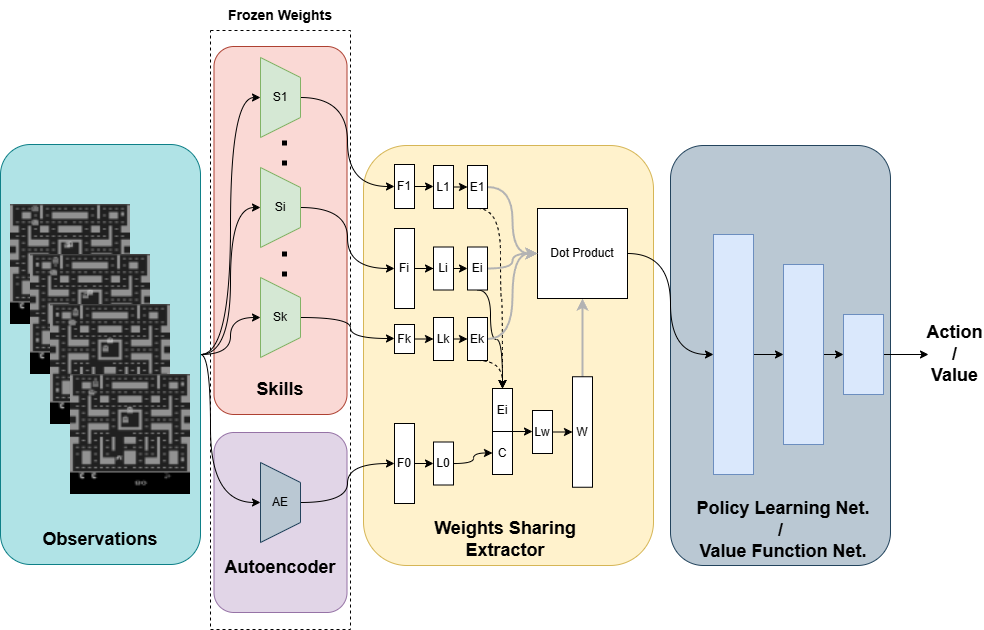
\includegraphics[width=\textwidth]{images/wsharing_module.png}
%     \end{center}
%     \caption{In Figure we show the Weights Sharing Attention Module. Each skill embedding $F_i$ is given as input to a different linear layer $L_i$. This is done to learn a representation of the skills and fix the size of the embeddings so that they are all equal. The same process is done for the autoencoder output so that the embedding for the context \textit{c} is created. At this point, for each skill, the context vector is concatenated with the embedding $E_i$ of a skill defining the input for the linear layer $L_w$ that will return the weight for the specific skill $w_i$, thus constituting the vector of weights \textbf{W}. Finally, the weighted sum $w_1*E_1 + w_2*E_2 + .... + w_k*E_k$ will be the new state representation to be passed to the agent. Each linear layer is followed by a ReLU layer.}
%     \label{fig:wsharingmodule}
% \end{figure}